\chapter{Miscellaneous Transformations}
\section{Fresnel Term - Schlick's approximation}
The \emph{Fresnel equations} describes the reflection and transmission of a electromagnetic wave at an interface. The Fresnel equation provides a reflection and transmission coefficients for waves. In Computer Graphics we often use the \emph{Schlick's approximation}. The specular reflection coefficient $R$ of the Fresnel equation can be approximated by:

\begin{equation}
 R(\theta) = R_0 + (1 - R_0)(1 - \cos \theta)^5
\label{eq:schlickapprox}
\end{equation}

and

\begin{equation*}
  R_0 = \left(\frac{n_1-n_2}{n_1+n_2}\right)^2
\end{equation*}

where $\theta$ is the angle between the viewing direction and the half-angle direction. This is equal to the halfway between the incident 
light direction and the viewing direction, i.e. $\cos \theta = (H \cdot V)$. $n_1$ $n_2$ are the refraction indices of the two medias. $R_0$ is the reflection coefficient for light incoming parallel to the normal (i.e., the value of the Fresnel term when $\theta = 0 \degree$ or minimal reflection). In Computer Graphics one of the interfaces is usually air, meaning that $n_1$ is approximately equal to 1.

\section{Spherical Coordinates and Space Transformation}
\label{sec:sphericalcoordinates}
\begin{figure}[H]
  \centering
  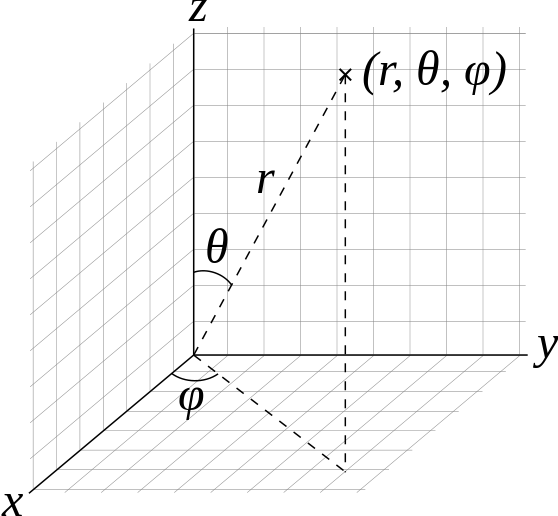
\includegraphics[scale=0.35]{sphericalcoordinates.png}
  \caption[Illustration of Spherical Coordinate System]{Illustration$\footnotemark$ of Spherical coordinates $(r,θ,φ)$ radius $r$, polar (inclination) angle $\theta$, and azimuthal angle $\phi$.}
  \label{fig:sphericalcoordinatesystem}
\end{figure}
\footnotetext{image source of figure $\ref{fig:sphericalcoordinatesystem}$ \texttt{http://en.wikipedia.org/wiki/Spherical\textunderscore coordinate\textunderscore system}} 

To define a \emph{spherical coordinate} system as shown in figure $\ref{fig:sphericalcoordinatesystem}$ we need two particular angles, the \emph{polar angle} $\theta$ and the \emph{azimuthal} $\phi$ plus a radius $r$. Then the Cartesian coordinates $(x,y,z)$ may be retrieved from their spherical coordinate representation as the following: $\forall \colvec[x]{y}{z} \in \mathbb{R}^3 : \exists r \in [0,\infty) \exists \phi \in [0,2\pi] \exists \theta \in [0,\pi] $ s.t.
\begin{equation*}
\colvec[x]{y}{z} = \colvec[r sin(\theta)cos(\phi)]{r sin(\theta)sin(\phi)}{r cos(\theta)}
\label{eq:sphericalcoordinates}
\end{equation*}

\label{sec:componentw}
From the definition $\ref{eq:uvw}$ of $(u,v,w)= -\omega_i - \omega_r$ and using spherical coordinates $\ref{eq:sphericalcoordinates}$, we get for $w$ the following identity:

\begin{align}
w 
&= -\omega_i - \omega_r \nonumber \\ 
&= -(\omega_i + \omega_r) \nonumber \\
&= -\left( cos(\theta_i)+cos(\theta_r) \right) 
\label{eq:sphericalomega}
\end{align}

and therefore $w^2$ is equal $(cos(\theta_i)+cos(\theta_r))^2$. 

\section{Tangent Space}
\label{sec:tangentspace}
The concept of performing a transformation into the \emph{tangent space} is used in order to convert a point between the world and and its local (tangent) space.  \\

We can think of the tangent space as a bumpy surface defined on a flat plane. If the normals of a fragment were defined in a world space coordinate system, we would have to rotate these normals every time the model is rotated - even when just for a small amount. Since lights, the camera and other scene primitives usually are defined in the world space coordinate system we would to have to rotate them according to every fragment position. This would require to apply countless many object-to-world transformations at a pixel level. The workaround for this issue is to transform all vertex primitives into tangent space in the vertex shader. \\

To make this point clear: Even we would rotate the cube as shown in figure $\ref{fig:cubeintangentspace}$, its tangent space axis will remain aligned w.r.t its face. This will save us from apply many space transformations on fragments.

\begin{figure}[H]
  \centering
  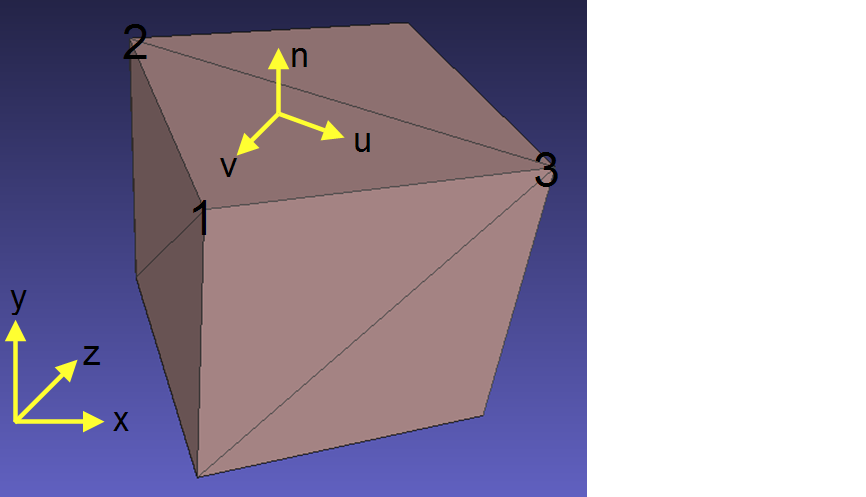
\includegraphics[scale=0.6]{tangentspace.png}
  \caption[Illustration of a Tangent Space]{Cube in world space $(x,y,z)$ showing the tangent-space $(u,v,n)$ of its face $(2,1,3)$}
  \label{fig:cubeintangentspace}
\end{figure}
